\section{序列的极限}
\label{sec:analysis-continuous-limits}

数列$1,1/2,1/3,\ldots$越来越接近$0$，数列$-1,1,-1,1,\ldots$则在两个值之间来回交替。
直觉上前者“有极限”，后者没有；但“越来越接近”需要精确的含义，否则无法判断更复杂的情形，
例如$(1+1/n)^n$或$\sum_{k\leq n}1/k$是否趋向某个数。
极限用误差条件给出这种含义：给定任意小的误差，后面的项是否都能落在这一误差范围内。

\label{sec:analysis-sequences-series-errors}

有了定义以后，还要回答两类问题：已知几个数列收敛时，怎样计算由它们组合出的数列的极限；
尚不知道极限值时，怎样从数列本身的性质保证极限存在。前者借助极限的运算法则与夹逼，
后者依靠单调有界、收敛子列和柯西准则，这三种判别都要用到第~\ref{sec:prelim-optimal-values-errors}节的确界原理。
本节先定义收敛并说明收敛数列有界，再建立存在性判别，然后讨论极限的唯一性、运算与夹逼，
最后用上、下极限描述不收敛数列尾部的上下边界。

\subsection{数列的收敛}

\paragraph{收敛与发散}
数列$(a_n)_{n\geq1}$是一列按正整数排列的实数。
“接近一个数”要同时约束后面的全部项，不能只看某几个位置：$((-1)^n)$的偶数项都等于$1$，
但奇数项始终离$1$有距离$2$，所以它不应算作趋于$1$。
只要求“各项与$a$的距离越来越小”也不够，例如$1+1/n$离$0$越来越近，却始终大于$1$。
合适的要求是：无论事先给定多小的正误差，从某一项起，后面\emph{每一项}与$a$的距离都小于这个误差。

若存在$a\in\mathbb R$，使每个$\varepsilon>0$都对应一个正整数$N$，满足
\[
 n\geq N\quad\Longrightarrow\quad |a_n-a|<\varepsilon,
\]
就称$(a_n)$\term{收敛}（converge）到$a$，$a$称为其极限，记作
$\lim_{n\to\infty}a_n=a$或$a_n\to a$。没有有限实数极限时，称数列发散（diverge）。
这里先任给误差$\varepsilon$，再选取$N$；选定以后，所有$n\geq N$都须满足要求。
$N$可以依赖于$\varepsilon$，误差要求越严格，所需的尾部起点通常越靠后；定义也不要求这个$N$唯一。
极限不要求某一项恰好等于$a$\scite{math-lebl-analysis1}。

例如对$a_n=1/n$，任给$\varepsilon>0$，取正整数$N>1/\varepsilon$，则$n\geq N$时
$|a_n-0|=1/n\leq1/N<\varepsilon$，所以$1/n\to0$。这样的整数$N$一定存在，因为正整数集合没有上界：
否则它有上确界$s$，而$s-1$不是上界，存在正整数$k>s-1$，于是正整数$k+1>s$，矛盾。

反过来，要说明$((-1)^n)$不收敛到任何$a$，只需取$\varepsilon=1$：
相邻两项相差$2$，不可能同时落在长度为$2$的开区间$(a-1,a+1)$内，所以没有$N$能使后面全部项满足要求。

图~\ref{fig:analysis-process-sequence-tail}把“全部尾部项”画成同一条误差带：选定起点以后，后面每一项都必须留在带内。
\begin{figure}[!htbp]
 \centering
 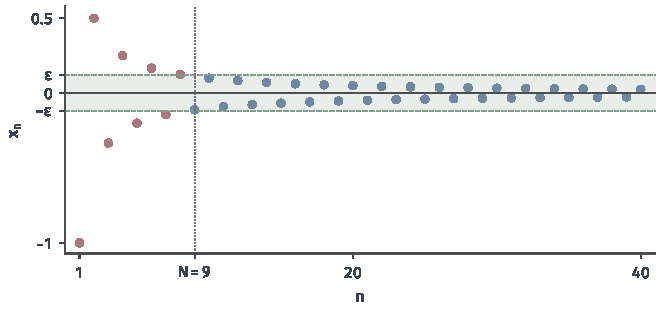
\includegraphics[width=112.0mm]{figures/00-shared/mathematical-preliminaries-upper/00-shared/matplotlib/chapter3-concept-processes/sequence-tail.pdf}
 \caption{数列$x_n=(-1)^n/n$的前40项。绿色带为$|x_n|<0.12$，取$N=9$后，所有$n\geq9$都在带内；蓝点标记这个尾部，红点标记之前的项。尾部条件针对无限多个$n$，其成立依据是$1/n\leq1/9<0.12$，不是只检查图中有限个点。}
 \label{fig:analysis-process-sequence-tail}
\end{figure}

\paragraph{收敛数列的有界性}
收敛的定义只控制尾部，但尾部之前只有有限个项，因此收敛数列必有界。
设$a_n\to a$，取$\varepsilon=1$，得到$N$使$n\geq N$时$|a_n-a|<1$，从而$|a_n|<|a|+1$。
令$M=\max\{|a_1|,\ldots,|a_{N-1}|,|a|+1\}$，便有$|a_n|\leq M$对所有$n$成立。

反向结论不成立，例如$((-1)^n)$有界却不收敛：有界性只限制取值范围，没有控制尾部是否还在振荡。
这一性质常以逆否形式使用：无界数列一定发散。下一小节将看到，
有界性再配合单调性，或者只要求选出一部分项，就能得到收敛的结论。

\subsection{数列的收敛判别}

定义收敛时需要指定一个候选极限，但很多数列的候选极限尚不明确。
下面依次利用变化方向、取值范围和尾部各项的互相接近来判断极限是否存在，并说明各自需要的条件。

\subsubsection{单调数列的收敛}
若对所有$n$都有$a_n\leq a_{n+1}$，称数列单调不减；
若总有$a_n\geq a_{n+1}$，称数列单调不增，两者统称为单调数列。

对于单调不减且有上界的数列，第~\ref{sec:prelim-optimal-values-errors}节的确界原理
为全部项提供一个最小上界；单调性则保证后面的项一直靠近它。
\begin{theorem}[单调有界收敛定理]
\label{thm:analysis-monotone-bounded-sequence}
设$(a_n)_{n\geq1}$为实数列。
若$a_n\leq a_{n+1}$对所有$n\geq1$成立，且存在$M\in\mathbb R$使$a_n\leq M$对所有$n\geq1$成立，则
\[
 \lim_{n\to\infty}a_n=\sup\{a_n:n\geq1\}\in\mathbb R.
\]
若$a_n\geq a_{n+1}$对所有$n\geq1$成立，且存在$m\in\mathbb R$使$a_n\geq m$对所有$n\geq1$成立，则
\[
 \lim_{n\to\infty}a_n=\inf\{a_n:n\geq1\}\in\mathbb R.
\]
\end{theorem}
\begin{proof}
设$a=\sup\{a_n:n\geq1\}$。给定$\varepsilon>0$，$a-\varepsilon$不是上界，
所以存在$N$使$a_N>a-\varepsilon$。单调性使$n\geq N$时都有
$a-\varepsilon<a_N\leq a_n\leq a$，这正是$a_n\to a$。
单调不增的情形对$-a_n$应用同一论证。
\end{proof}
证明中只有一处用到实数的\term{完备性}（completeness）：非空上有界的实数集合$\{a_n:n\geq1\}$有实数上确界。
两个条件都不能省去：$(n)$单调却无上界，$((-1)^n)$有界却不单调。
结合收敛数列的有界性可知，单调数列收敛当且仅当它有界。

\subsubsection{有界数列的子序列收敛}
数列可能整体不收敛，但其中一些项仍有共同的趋向。保持原有次序选出一部分项，
得到子序列（subsequence），也称子列：若$n_1<n_2<\cdots$为严格递增的正整数列，
则$(a_{n_k})_{k\geq1}$为$(a_n)$的子序列。由归纳可知$n_k\geq k$。

收敛数列的每个子序列都收敛到同一极限：若$n\geq N$时$|a_n-a|<\varepsilon$，
则$k\geq N$时$n_k\geq k\geq N$，同一误差界仍然适用。
反过来，一个子序列收敛不能保证原数列收敛；$((-1)^n)$的偶数项恒为$1$，奇数项恒为$-1$。

有界数列未必收敛，但有界性能保证从中选出一个收敛子序列。
这一结论称为Bolzano--Weierstrass定理，随后将用它证明柯西条件足以保证实数列收敛。
\begin{theorem}[Bolzano--Weierstrass定理]
\label{thm:analysis-bounded-subsequence}
设$(a_n)_{n\geq1}$为实数列。若存在$M\geq0$使$|a_n|\leq M$对所有$n\geq1$成立，
则存在严格递增的正整数列$n_1<n_2<\cdots$和$a\in\mathbb R$，使
\[
 \forall\varepsilon>0,\quad\exists K\in\{1,2,\ldots\},\quad
 k\geq K\Longrightarrow |a_{n_k}-a|<\varepsilon.
\]
即$a_{n_k}\to a$。
\end{theorem}
\begin{proof}
从包含全部项的闭区间$I_0=[-M,M]$出发，将它平分，两半中至少有一半含有无穷多个下标对应的项；
选出这一半，再重复平分与选择，得到嵌套闭区间$I_0\supseteq I_1\supseteq\cdots$，
其中$I_k=[l_k,r_k]$含有无穷多项，长度为$2M\cdot2^{-k}$。
由$2^k\geq k+1$，这些长度至多为$2M/(k+1)$，因而趋于零；这里不必先用后面的等比数列极限。
由于每个$I_k$都含有无穷多项，可以依次选取下标$n_1<n_2<\cdots$，使$a_{n_k}\in I_k$。

再确定子序列的极限。各左端点$l_k$单调不减，而由嵌套性，每个$r_j$都是全部左端点的上界。
由确界原理，$c=\sup_k l_k$存在，并满足$l_k\leq c\leq r_k$对每个$k$成立。
给定$\varepsilon>0$，先选$K$使$r_K-l_K<\varepsilon$；
当$k\geq K$时，$a_{n_k}\in I_k\subseteq I_K$，且$c\in I_K$，所以$|a_{n_k}-c|\leq r_K-l_K<\varepsilon$。
\end{proof}

\subsubsection{柯西数列的收敛}
单调条件并不适用于所有收敛数列。若还不知道候选极限，可以检查尾部各项是否彼此接近。
满足
\[
 \forall\varepsilon>0,\quad\exists N,\quad
 \forall m,n\geq N,\quad |a_m-a_n|<\varepsilon
\]
的数列称为\term{柯西数列}（Cauchy sequence）。对实数列，这个条件与收敛等价。
\begin{theorem}[柯西收敛准则]
\label{thm:analysis-cauchy-convergence}
设$(a_n)_{n\geq1}$为实数列。存在$a\in\mathbb R$使$a_n\to a$，当且仅当
\[
 \forall\varepsilon>0,\quad\exists N\in\{1,2,\ldots\},\quad
 \forall m,n\geq N,\quad |a_m-a_n|<\varepsilon.
\]
\end{theorem}
\begin{proof}
每个收敛实数列都是柯西数列：若$n\geq N$时$|a_n-a|<\varepsilon/2$，则对$m,n\geq N$，
$|a_m-a_n|\leq|a_m-a|+|a_n-a|<\varepsilon$。

反过来，柯西条件先保证数列有界，论证与收敛数列的有界性相同，只是把极限换成尾部中的一项：
取误差$1$，所有$n\geq N$都满足$|a_n-a_N|<1$，前面有限个项另取最大绝对值即可。
由Bolzano--Weierstrass定理，可取子序列$a_{n_k}\to a$。

给定$\varepsilon>0$，选$N$使任意$m,n\geq N$满足$|a_m-a_n|<\varepsilon/2$，
再选一个$k$，使$n_k\geq N$且$|a_{n_k}-a|<\varepsilon/2$。
于是每个$n\geq N$都有
$|a_n-a|\leq|a_n-a_{n_k}|+|a_{n_k}-a|<\varepsilon$。
\end{proof}
这一准则的充分性通过收敛子列，仍然依赖实数的确界原理。

验证柯西条件时，可把两个较晚的项之间的距离估计为逐步变化的总和。对$m>n$，
\begin{equation}
 |a_m-a_n|\leq\sum_{k=n}^{m-1}|a_{k+1}-a_k|.
\label{eq:analysis-cauchy-tail-bound}
\end{equation}
仅有相邻差趋零还不够，因为中间的步数也在增加，必须控制整段和。
例如$a_1=0$、$a_{k+1}-a_k=1/k$时，每一步都趋零，但$a_{2n}-a_n=\sum_{k=n}^{2n-1}1/k$共有$n$项，
每项都大于$1/(2n)$，所以$a_{2n}-a_n>1/2$，它不是柯西数列，因而发散。
这里的$a_{n+1}$正是第~\ref{sec:analysis-series}节调和级数的前$n$项和：每一项都变小，累计却不稳定。

\subsection{极限的基本性质}

前面的判别给出了保证收敛的条件。现在假定实数列已经收敛，先说明极限唯一，
再分别计算和、差、数乘、积与商的极限，最后说明怎样用上下界夹逼求极限。
这些运算法则都以有限极限存在为前提，不能代替收敛性的判别。

\paragraph{极限的唯一性}
收敛数列的极限是唯一的。若$a\neq b$都是极限，
取$\varepsilon=|a-b|/3$，充分靠后的项应同时满足
$|a_n-a|<\varepsilon$和$|a_n-b|<\varepsilon$；
三角不等式却给出$|a-b|\leq|a-a_n|+|a_n-b|<2|a-b|/3$，矛盾。
因此记号$\lim_{n\to\infty}a_n$表示一个确定的数。

\paragraph{和的极限}
实际计算时，一个数列常由几个已知数列相加得到。设$a_n\to a$、$b_n\to b$，其中$a,b\in\mathbb R$，则
\[
 \lim_{n\to\infty}(a_n+b_n)=a+b.
\]
因为$|(a_n+b_n)-(a+b)|\leq|a_n-a|+|b_n-b|$，
只需让两个误差分别小于$\varepsilon/2$，便能使和的误差小于$\varepsilon$。

\paragraph{差的极限}
相减时也可以分别控制两列数的误差。在同样的有限收敛条件下，
\[
 \lim_{n\to\infty}(a_n-b_n)=a-b.
\]
这来自$|(a_n-b_n)-(a-b)|\leq|a_n-a|+|b_n-b|$，取尾部起点使右侧两项各小于$\varepsilon/2$即可。

\paragraph{数乘的极限}
把每一项乘以固定的实数$c$，只会把误差乘以$|c|$，所以
\[
 \lim_{n\to\infty}ca_n=ca.
\]
$c=0$时结论直接成立；$c\neq0$时，把原数列误差控制在$\varepsilon/|c|$以内即可。

\paragraph{积的极限}
乘积的误差还包含一个变化的因子，需要用到收敛数列的有界性。若$a_n\to a$、$b_n\to b$，则
\[
 \lim_{n\to\infty}a_nb_n=ab.
\]
取$M\geq1$使所有$|a_n|\leq M$，把误差拆成两部分：
\[
 |a_nb_n-ab|=|a_n(b_n-b)+b(a_n-a)|\leq M|b_n-b|+|b|\,|a_n-a|.
\]
让$|b_n-b|<\varepsilon/(2M)$、$|a_n-a|<\varepsilon/[2(|b|+1)]$同时成立，右侧便小于$\varepsilon$。

\paragraph{商的极限}
除法还须避免分母趋零。若$a_n\to a$、$b_n\to b$且$b\neq0$，则充分靠后的$b_n\neq0$，并且
\[
 \lim_{n\to\infty}\frac{a_n}{b_n}=\frac ab.
\]
事实上，取误差$|b|/2$，可知充分靠后的$|b_n|\geq|b|/2$，于是
$|1/b_n-1/b|=|b_n-b|/(|b_n||b|)\leq2|b_n-b|/|b|^2$，右侧趋于零；
前面有限个项不影响极限，再对$a_n\cdot(1/b_n)$用乘积规则即得结论。
例如将分子分母同除以$n$，得$n/(n+1)=1/(1+1/n)\to1$。
分母趋于零时不能套用此式：$0/0$与$\infty-\infty$一样，都不是可以直接计算的数值。

\paragraph{夹逼定理}
有时中间数列不断振荡，直接控制它的误差并不方便，但可以分别找到上下界。
若上下两列最终都靠近同一有限值，中间数列便被限制在同一误差范围内。
\begin{theorem}[夹逼定理]
\label{thm:analysis-sequence-squeeze}
设$(a_n)$、$(b_n)$、$(c_n)$为实数列。若存在正整数$N_0$使
\[
 \forall n\geq N_0,\qquad a_n\leq c_n\leq b_n,
\]
并且存在$\ell\in\mathbb R$满足
$\lim_{n\to\infty}a_n=\lim_{n\to\infty}b_n=\ell$，则
$\lim_{n\to\infty}c_n=\ell$。
\end{theorem}
\begin{proof}
任给$\varepsilon>0$，由两端收敛可选正整数$N_1,N_2$，使
$n\geq N_1$时$|a_n-\ell|<\varepsilon$，$n\geq N_2$时$|b_n-\ell|<\varepsilon$。
取$N=\max\{N_0,N_1,N_2\}$，则每个$n\geq N$都有
\[
 \ell-\varepsilon<a_n\leq c_n\leq b_n<\ell+\varepsilon.
\]
所以$|c_n-\ell|<\varepsilon$，按定义即$c_n\to\ell$。
\end{proof}
例如$-1/n\leq(\sin n)/n\leq1/n$，所以$(\sin n)/n\to0$。

一个反复使用的例子是$|r|<1$时$r^n\to0$。$r=0$时直接成立；
若$0<|r|<1$，写$1/|r|=1+h$，其中$h>0$。
先用归纳法证明$(1+h)^n\geq1+nh$：$n=1$时取等号；若它对$n$成立，则
$(1+h)^{n+1}\geq(1+nh)(1+h)=1+(n+1)h+nh^2\geq1+(n+1)h$。
因此$0<|r|^n\leq1/(1+nh)<(1/h)\cdot(1/n)\to0$，
再对$-|r|^n\leq r^n\leq|r|^n$用夹逼定理，得到$r^n\to0$。

这回答了章首关于等比递推~\eqref{eq:prelim-geometric-recurrence}的问题：
$|\rho|<1$时$e^{(t)}=\rho^te_0\to0$。另几种情形同样可以判断：设$e_0\neq0$，
$\rho=1$时各项恒为$e_0$；$\rho=-1$时各项在$\pm e_0$间交替，不收敛；
$|\rho|>1$时，同一不等式给出$|\rho|^t\geq1+th$（其中$|\rho|=1+h$），数列无界，因而发散。

\subsection{数列的上极限与下极限}
数列不收敛时，仍可考察其尾部的上下边界。
为记录无界的趋向，约定$a_n\to+\infty$表示对每个实数$M$，充分大的$n$都满足$a_n>M$；
$a_n\to-\infty$则要求最终都有$a_n<M$。
这两个符号不是有限实数极限，$\overline{\mathbb R}=\mathbb R\cup\{-\infty,+\infty\}$称为扩展实数，
其中$\infty-\infty$没有定义。

逐渐舍去前项时，尾部下界只会上升，尾部上界只会下降，因此可以分别用单调数列的极限记录它们。
\begin{definition}[数列的上极限与下极限]
\label{def:analysis-liminf-limsup}
对扩展实数列$(a_n)$，定义
\[
 \liminf_{n\to\infty}a_n
 =\lim_{n\to\infty}\inf_{k\geq n}a_k,
 \qquad
 \limsup_{n\to\infty}a_n
 =\lim_{n\to\infty}\sup_{k\geq n}a_k.
\]
右侧尾部下确界随$n$单调不减，尾部上确界随$n$单调不增，故两者的极限均在扩展实数中存在。
\end{definition}
这里的单调极限允许取$\pm\infty$：单调不减的数列有上界时由单调有界收敛定理收敛，
无上界时对每个$M$都有某一项超过$M$，此后各项也超过$M$，即趋于$+\infty$；单调不增的情形同理。

例如$((-1)^n)$的下极限为$-1$、上极限为$1$，通常极限不存在。
总有$\liminf a_n\leq\limsup a_n$，因为每个尾部的下确界不超过同一尾部的上确界。
二者同为有限值$a$当且仅当$a_n\to a$。若二者都等于$a$，则对给定$\varepsilon>0$，
充分靠后的尾部下确界大于$a-\varepsilon$、尾部上确界小于$a+\varepsilon$，夹在中间的每个尾部项都满足$|a_n-a|<\varepsilon$；
反之若$a_n\to a$，则$n\geq N$时尾部全落在$(a-\varepsilon,a+\varepsilon)$内，尾部的上下确界都在$[a-\varepsilon,a+\varepsilon]$中。
二者同为$+\infty$或$-\infty$时则对应上述无穷极限，仍应与有限实数收敛区别。

对有界实数列，上、下极限还可以由子序列达到。记$L=\limsup a_n$。
对每个$j$，先取足够晚的起点，使其后的尾部上确界小于$L+1/j$；
由于每个尾部的上确界都不小于$L$，这一尾部中又有某项大于$L-1/j$。
在下标超过前次所选下标的位置选出这样的项$a_{n_j}$，便有$|a_{n_j}-L|<1/j$，从而$a_{n_j}\to L$。下极限同理。

\FloatBarrier
